%
%	WISS 2013サンプルファイル (未来ビジョンテンプレート, 最後数行空き問題解決バージョン)
%
%	2010/07/12 Ver 1.0 秋田 純一
%	2010/08/04 Ver 1.1 後藤 真孝
% 	2011/09/27  Ver 1.4 渡邊 恵太 (協力:五十嵐悠紀)


\documentclass[twoside]{wiss}

\usepackage{ascmac}
\usepackage[dvips]{graphicx}
\usepackage{nidanfloat} %% appended in WISS2010 for Future Vision (2010/7/7:akita)
\usepackage{multicol}
%\usepackage{color,array}
%\usepackage{boxedminipage}

%% balance.styを追加 (2012/9/27:watanabe, Igarashi)
\usepackage{balance}    %% 最後のページの高さを揃えるために追加  (2012/9/27:watanabe, Igarashi)
%%% 最後のページの2段組の高さを揃える.\balanceを入れる.
%%% そろえたくないときは、\nobalance


%% Here.stylを追加
\usepackage{here}

\def\system{SuperIME}
\def\papertitle{\system: IMEによるテキスト編集機能の統合}

\journalhead{\papertitle} %%%%%% ←← 著者において必ず記入すること

\begin{document}

\title{\papertitle}
\etitle{}%2012年では英文タイトルは廃止されました.記入しないでください.
%
%注意
%
%
% WISS2013ではダブルブラインドとなりました.投稿時には氏名と所属は記入しないでください.
\author{匿名で査読を行うため著者名なし
	\affil{匿名で査読を行うため所属名なし}}

\begin{abstract}
計算機上で様々なテキストエディタが利用されているが、
システムごとに編集方法や編集機能が異なっているのが不便である。
本論文では、各国語入力のためにOSに用意されているIME(Input Method Editor)機能を利用することにより、
あらゆるテキストエディタにおいて同じ操作によるテキスト編集を可能にする方法を提案する。
我々の手法を利用すると,異なるテキストエディタ上での編集操作が共通化されるだけでなく、
テキスト編集時に便利な様々な機能をあらゆるエディタで利用することが可能になる。
\end{abstract}


\maketitle

\section{はじめに}

計算機上でテキストを編集するために様々なテキストエディタが利用されている。
文書を作成するときはワープロを利用し、
メールを書くにはメールクライアントを利用し、
文字端末でのプログラム開発にはvimやEmacsを利用し、
IDEを利用した開発では付属のエディタを利用し、
ネット上でテキストを扱うにはブラウザのテキストフォームを利用するといったように、
場合によって異なるエディタが利用されている。

エディタの機能や操作体系はシステムごとに異なっているのが普通である。
ブラウザやワープロでテキストを1行消したい場合は
マウスで行全体を選択してから削除キーを押せばよいが、
vimでは「d」キーを2回タイプして消すことが多く、
EmacsではCtrl-Kキーがよく使われている。
Emacsに慣れたユーザがワープロ上でもCtrl-Kで行を消去したいと思っても、
そういう機能は用意されていないのが普通であるし、
機能拡張が可能なシステムを利用している場合でも、
操作体系を完全に同じにすることは難しい。
%
あらゆるエディタの操作を統一することは難しいが、
様々なエディタで共通に利用できるソフトウェア層を
ユーザとアプリケーションの間に置くことができれば
異なるエディタの編集操作をある程度共通化できる可能性がある。

現在のパソコンには IME(Input Method Editor) と呼ばれる文字入力機構が用意されており、
様々な言語のテキスト入力に利用されている。
IMEはエディタなどとは独立したソフトウェアであり、
ユーザのすべてのキー入力を受け取って
各国語に変換した結果をアプリケーションに送出する。
IMEはあらゆるアプリケーションで共通に利用されるので、
たとえば日本語入力用のIMEを利用すれば、
Emacs でもブラウザでも IDE でも同じ操作で日本語を入力できる。
IMEは一般には各国語入力のみのために利用されているが、
テキストの挿入/移動/削除といった編集操作もIMEが受け持つようにすれば、
様々なエディタ上で同じ操作で編集を行なうことが可能になる。
%
Mac上の様々なテキストエディタにおいて
同じキー操作でテキスト編集を可能にする{\system}システムについて述べる。



\section{実装例}

MacRubyで記述された IME である「Gyaim」に様々な編集機能を追加したものを
利用した編集作業の例を示す。一般にIME はアルファベット以外の文字を入力
するときだけ有効にするのが普通であるが、ここでは Gyaim を 常に有効にし
ておくことによりあらゆるキー入力を Gyaim が取得している。

\subsection{ブロック移動}

テキストの一部を別の場所に移動したいことは多いが、
エディタによって操作方法が全く異なっている。
たとえばEmacsでテキストを移動させたい場合は、
移動する領域をキー操作によって指定してから削除/コピーし、
カーソルを移動してペーストするという手順を利用するが、
ブラウザの編集領域でテキストを移動させたい場合は、
マウスで領域を指定した後で領域をドラッグして別の位置に移動するのが基本である。
テキスト移動のような基本操作でもエディタごとに操作が異なっているのが不便であるが、
Gyaimを利用するとあらゆるエディタで同じ操作でテキストを移動することができる。

図\ref{move1}はMac OSに標準でインストールされている、「テキストエディット」で編集中のテキストである。

\begin{figure}[H]
\centerline{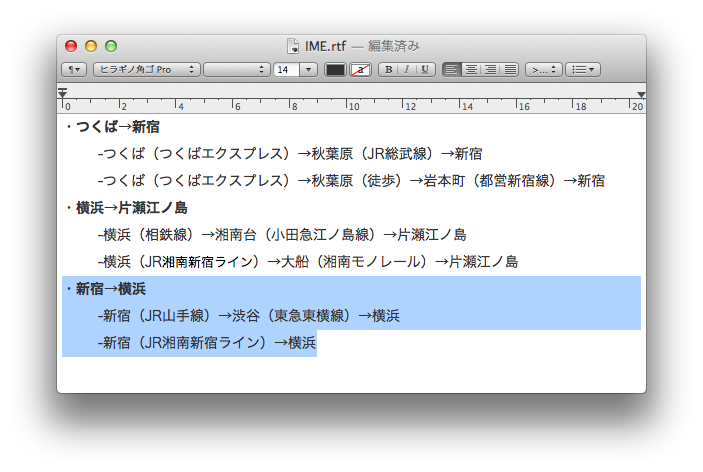
\includegraphics[width=70mm,bb=0 0 703 472]{figures/block2.png}}
\caption{ブロック移動前の状態.}
\label{move1}
\end{figure}

ここでShift+↑キーを押すとテキストは図\ref{move2}のように変化する。

\begin{figure}[H]
\centerline{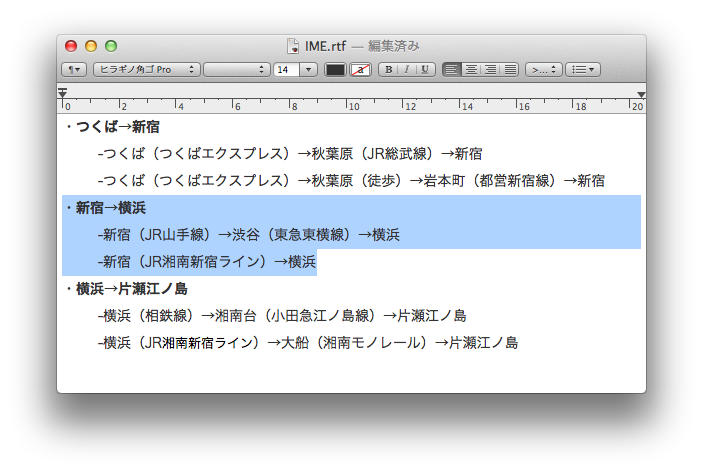
\includegraphics[width=70mm,bb=0 0 703 472]{figures/block3.png}}
\caption{Shift+↑キーを押した後の状態.}
\label{move2}
\end{figure}

図\ref{move3}はブラウザ上でGoogle Docsのテキストを編集しているところである。
ここでShift+↑キーを二度押すと、テキストは図\ref{move4}のように変化する。

\begin{figure}[H]
\centerline{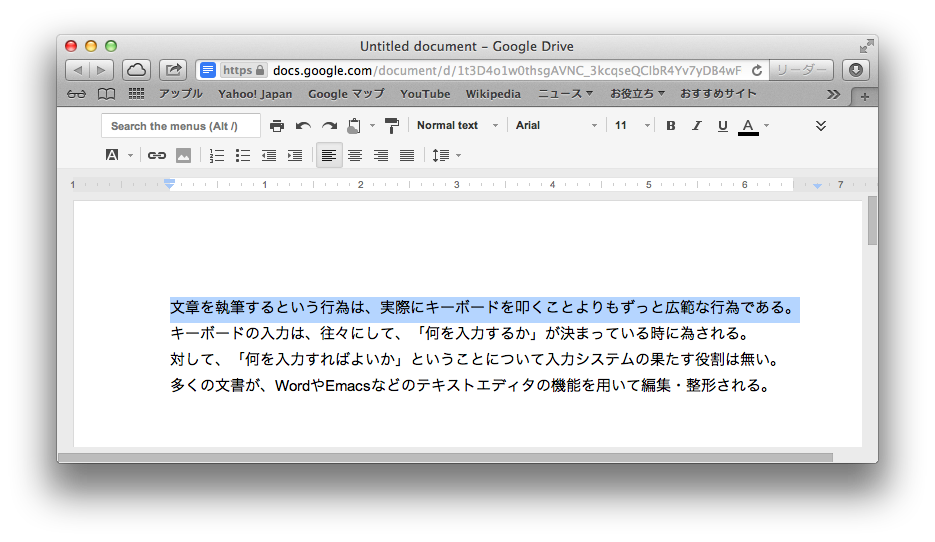
\includegraphics[width=70mm,bb=0 0 935 542]{figures/block4.png}}
\caption{ブロック移動前の状態.}
\label{move3}
\end{figure}

\begin{figure}[H]
\centerline{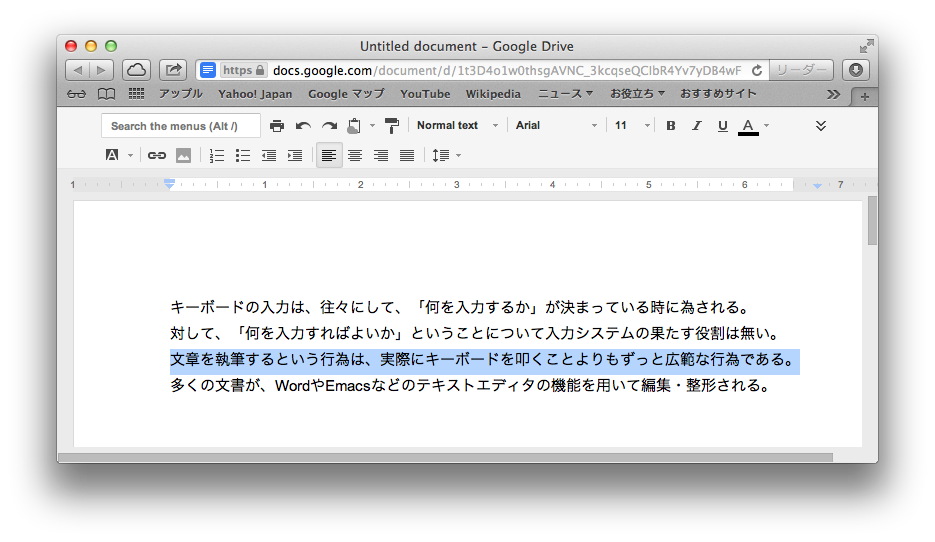
\includegraphics[width=70mm,bb=0 0 935 542]{figures/block5.png}}
\caption{キーを押した後の状態.}
\label{move4}
\end{figure}

このように、あらゆるエディタにおいて同じ操作でブロック移動を行なうことができることがわかる。

\subsection{連続インデント}

前述したブロック移動は、インデントを調整する機能も備えている。
プログラミングを行なっている時だけでなく、
普通のテキストを編集している場合でも
行頭の空白やタブの量を調整するインデント処理は頻繁に行われるが、
自動的にインデントを行うエディタもあれば、
コマンドを打ち込まなければならないものもあり、
そのような調整機能を持っていないエディタも多い。
Gyaimを利用すると、あらゆるエディタや入力フィールドでブロック移動と同時にインデントが自動で行われる。

図\ref{indent1}は、Xcode上でPythonプログラムを書いている例である。
Xcodeは、Objective-CやRubyなどの言語で自動インデントの機能を備えているが、Pythonには対応していない。
たとえば、図\ref{indent1}のようなテキストに対して
図\ref{indent2}のように移動させたいブロックを選択し、Shift+↓キーを入力することで、テキストは図\ref{indent3}のように変化する。

\begin{figure}[H]
\centerline{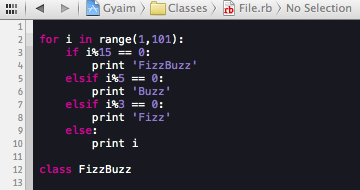
\includegraphics[width=70mm,bb=0 0 360 190]{figures/indent1.png}}
\caption{ブロック移動前の状態}
\label{indent1}
\end{figure}

\begin{figure}[H]
\centerline{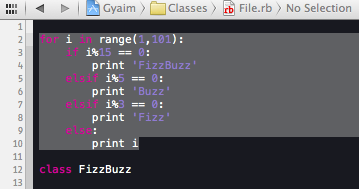
\includegraphics[width=70mm,bb=0 0 360 190]{figures/indent2.png}}
\caption{テキストを選択した状態}
\label{indent2}
\end{figure}

\begin{figure}[H]
\centerline{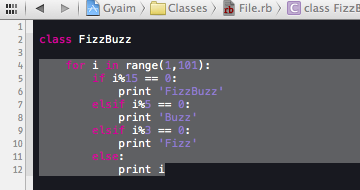
\includegraphics[width=70mm,bb=0 0 360 190]{figures/indent3.png}}
\caption{ブロック移動後の状態}
\label{indent3}
\end{figure}

このように、あらゆるエディタにおいて、ブロック移動を行う際に適切な空白とタブを自動で補完することができる。

\subsection{単語置換}
テキスト編集における単語の検索と置換は、多くのエディタが備えている機能であるが、
その操作方法は異なっている。また、Webブラウザや、
DTPソフトなどでテキストを扱うとき、
検索や置換といった機能は用意されていない。
ブラウザに入力したテキストを、エディタにコピーして編集操作を行うといった作業、あるいはその逆といった作業をGyaimにより共通化することが出来る。

以下にGyaimによる単語置換の例を示す。図\ref{search1}のように入力語と置換語をテキストエリアに打ち込み、任意に設定したファンクションキーを押すと、
テキストは図\ref{search2}のように置換される。

\begin{figure}[H]
\centerline{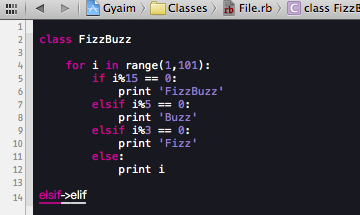
\includegraphics[width=70mm,bb=0 0 360 215]{figures/search_replace1.png}}
\caption{単語置換操作の例}
\label{search1}
\end{figure}

\begin{figure}[H]
\centerline{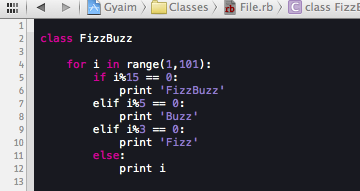
\includegraphics[width=70mm,bb=0 0 360 191]{figures/search_replace2.png}}
\caption{単語置換後の状態}
\label{search2}
\end{figure}

このように、あらゆるエディタ上で検索と置換が可能である。

\subsection{Emacs Lisp}
Emacsにおいてはlisp拡張を導入することでエディタの機能を拡張することが出来るが、これらのスクリプトをIME上に実装することで、他のエディタ上でもこれらの有用な拡張機能を動作させることができる。

以下にGyaimによる \cite{Dynamic Macro}の例を挙げる。
Dynamic Macroは、入力の繰り返しを自動化するEmacs拡張である。
図\ref{dynamic1}のように、ユーザの入力操作が繰り返しになっているとき、任意に設定したファンクションキーを押すと、テキストは図\ref{dynamic2}のように編集される。

\begin{figure}[H]
\centerline{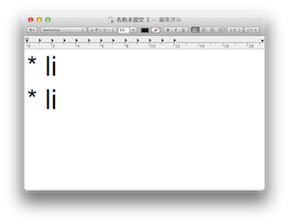
\includegraphics[width=80mm,bb=0 0 360 190]{figures/dynamic1.png}}
\caption{Dynamic Macro機能を使用する前のテキスト}
\label{dynamic1}
\end{figure}

\begin{figure}[H]
\centerline{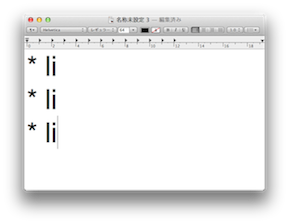
\includegraphics[width=80mm,bb=0 0 360 190]{figures/dynamic2.png}}
\caption{Dynamic Macro機能を使用した後のテキスト}
\label{dynamic2}
\end{figure}


以下はGyaimのDynamic Macro機能をブラウザのアドレスバー上で実行した例である。
図\ref{dynamic3}のように、ユーザの入力に"abc"が繰り返されているとき、任意に設定したファンクションキーを押すと、テキストは図\ref{dynamic4}のように編集される。

\begin{figure}[H]
\centerline{
\includegraphics[width=70mm,bb=0 0 360 50]{figures/dynamic3.png}}
\caption{Dynamic Macro機能を使用する前のテキスト}
\label{dynamic3}
\end{figure}

\begin{figure}[H]
\centerline{
\includegraphics[width=70mm,bb=0 0 360 50]{figures/dynamic4.png}}
\caption{Dynamic Macro機能を使用した後のテキスト}
\label{dynamic4}
\end{figure}





\section{実装}
Gyaim は MacRuby で記述された Mac 用の IME であり、ソースが 500 行程度とコンパクトであるにもかかわらず、他の IME に見られない機能を実装しており、本論文のような実験も容易である。

\subsection{MacRuby}
MacRuby は、Mac 用のアプリケーションを開発するために拡張された Ruby 実行環境であり、Mac の Objective-C ライブラリを Ruby で扱うことが出来る。
Gyaim では、日本語などの入力を補助するフレームワークである InputMethodKit Framework を MacRuby から呼び出すことによって基本的な IME の機能を実装している。

しかし、ブロック移動やインデントの処理をあらゆる テキストエリアで行うためには、テキストフィールドに 入力されている全文をIMEが取得する必要があり、InputMethodKit はこの機能を備えていない。Gyaim では、AppleScript などを併用することによりこの問題を解決したが、実装には課題が残っている。


\section*{謝辞}

謝辞は、ブラインドレビューのため、投稿時には削除すること.
カメラレディ時に、必要があれば追加すること.

Dynamic Macro system\cite{DynamicMacro}
\cite{texteditors.org}
\cite{Kawada:WP}
\cite{Mori:WordProcessor}
\cite{Doi:STARS}
\cite{Doi:COLING98}
\cite{texteditors.org}
\cite{Li:1lineKB}\cite{MacKenzie:H4Writer}\cite{Rick:VirtualKB}
\cite{Dietz:PressureKB}\cite{Harrison:Skinput}\cite{Murase:CameraKB}\cite{Wigdor:TiltKB}
\cite{Tesler:CopyPaste}.
\cite{Masui:Goldfish}\cite{PickAndDrop}.

% \section{参考文献}

{\scriptsize
\bibliographystyle{jwiss}
\bibliography{wiss2013_gyaim}
}

%%
%%	参考文献
%%
% \begin{thebibliography}{1}

% \bibitem{wiss} WISSホームページ.  http://www.wiss.org/.

% \bibitem{aoki1999} H.~Aoki, B.~Schiele, and A.~Pentland.  Realtime
% Personal Positioning System for Wearable Computers.  In
% \emph{Proceedings of the 3rd IEEE International Symposium on Wearable
% Computers}, pp. 37--43, 1999.

% \bibitem{rekimoto2000} 暦本 純一.  まえがき:WISS2000について.  インタラ
% クティブシステムとソフトウェアVIII, pp. i--ii. 近代科学社, 2000.

% \end{thebibliography}


%%% 未来ビジョンの枠が変なところに出る

% %%%%%%%%%%%%%%%%%%%%%%%%%%%%%%%%%%%%%%%%%%%%%%%%%%%%%%%%%%%%%%%%%%%%%
% %%%%%%%%%%%%%%%%%%%%%%%%%%%%%%%%%%%%%%%%%%%%%%%%%%%%%%%%%%%%%%%%%%%%%
% %% WISS2012では,「未来ビジョン」は以下のように,本文と同様の2段組形式で記載する.
% %% 図を用いても良いが,枠のサイズ(縦93mm)を変更してはならない.
% %% (WISS2010では,縦118mmでしたのでご注意下さい)


% \begin{figure*}[!b]
% \setlength{\unitlength}{1mm}\fboxrule=0.5pt

% \vspace{-93mm} %% 未来ビジョンの枠が下がってしまうのを防ぐ WIS2012 カメラレディテンプレで追加  (2012/9/27:watanabe, Igarashi)

% % 未来ビジョンの枠の描画
% \begin{center}
% \framebox[0.95\textwidth]{
% \begin{minipage}{0mm}\begin{picture}(0,91)(0,0)\end{picture}\end{minipage}
% }
% \end{center}
% \vspace*{-93mm}	% 未来ビジョンの枠の縦幅分だけ戻す

% % 未来ビジョンの内容
% \newbox\FUTURE
% \setbox\FUTURE=\vbox{
% \begin{minipage}[b]{0.9\textwidth}
% \begin{multicols}{2}	% 二段組にする
% \section*{未来ビジョン}
% \setlength{\parindent}{10pt}	% 段落先頭の字下げ

% % % % % % % % % % % % % % % % % % % % % % % % % % % % % % %
% %	   未来ビジョンは,下記に記入して下さい		  %
% % % % % % % % % % % % % % % % % % % % % % % % % % % % % % %

% \vspace*{-1mm}

% % フォントサイズ指定
% \normalsize
% %\large
% %\small\setlength{\baselineskip}{12pt}
% %\footnotesize\setlength{\baselineskip}{12pt}

% 未来ビジョン
% % % % % % % % % % % % % % % % % % % % % % % % % % % % % % %
% %	   未来ビジョンは,上記に記入して下さい		  %
% % % % % % % % % % % % % % % % % % % % % % % % % % % % % % %

% \end{multicols}
% \end{minipage}
% }

% % 未来ビジョンの内容の描画
% \newlength{\FUTUREHT}
% \setlength{\FUTUREHT}{\the\ht\FUTURE}	% 未来ビジョンの内容の縦幅保存
% %\typeout{\the\wd\FUTURE}
% %\typeout{\the\ht\FUTURE}
% \hspace*{0.045\textwidth}	% 未来ビジョンの内容の横位置調整
% \box\FUTURE
% %\typeout{\the\FUTUREHT}
% \vspace*{-\the\FUTUREHT}	% 未来ビジョンの内容の縦幅分だけ戻す
% \vspace*{-10.9mm}		% 微調整

% % 未来ビジョンの枠の領域の再確保(これがないと枠が下に沈み込む)
% \begin{center}
% \fboxrule=0pt
% %\fboxrule=2pt	% デバッグ用: コメントアウトをやめて,同じ位置に枠が出るか?
% \framebox[0.9\textwidth]{
% \begin{minipage}{0mm}\begin{picture}(0,91)(0,0)\end{picture}\end{minipage}
% }
% \end{center}
% \end{figure*}

%%%%%%%%%%%%%%%%%%%%%%%%%%%%%%%%%%%%%%%%%%%%%%%%%%%%%%%%%%%%%%%%%%%%%
%%%%%%%%%%%%%%%%%%%%%%%%%%%%%%%%%%%%%%%%%%%%%%%%%%%%%%%%%%%%%%%%%%%%%
\end{document}
